\chapter{Machine Translation by Pattern Matching}\label{chap:overview}

\begin{quote}
	{\em 
	\begin{itemize}
		\item[\rm Calvin:] You can't just turn on creativity like a faucet. You have to be in the right mood.
		\item[\rm Hobbes:] What mood is that?
		\item[\rm Calvin:] Last-minute panic.
	\end{itemize}
	}
	\begin{flushright}
		--Bill Watterson
	\end{flushright}
\end{quote}

Statistical MT models typically contain many millions of parameters.
So far in our discussion, the implications of this have been abstract.
We now turn our attention to the implementation of translation models.
Our main concern will be efficient representation of and access to 
model parameters.

The number of model parameters depends on training data size and
model complexity.  Trends toward larger data and more articulated models 
place increasing pressure on implementations.  If we rely on direct
representation of a model trained on large data, it is already quite easy to create a
translation system that exhausts the main memory of the commodity hardware
on which most research systems are developed.

\citet{Callison-Burch:2005:acl} and \citet{Zhang:2005:eamt} introduced
an alternative that we call {\em translation by pattern matching}.
It relies on indirect representation of the
translation model, using the training data itself as its proxy.  This
representation is compact.  More importantly, it is independent of model size,
enabling us to scale to arbitrarily large models (Chapter~\ref{chap:scaling}).   
Rather than enumerate and compute all parameters of the model offline, translation by pattern
matching works by efficiently searching for relevant sections of the training
data at runtime, and extracting and computing the needed parameters
from these sections.  This efficient search is based on algorithms
for pattern matching.

Although \citet{Callison-Burch:2005:acl} and \citet{Zhang:2005:eamt}
lay the foundation for pattern matching, there are some open problems.
They did not demonstrate that they could match---let alone 
exceed---the performance of a common baseline system.  In fact, a few elements
of their approach appear to be incompatible with other methods used
in the state of the art.  Therefore, it is unclear whether 
translation by pattern matching is even a viable replacement for 
direct representation.  In this chapter, we answer this question affirmatively.

This chapter is organized as follows.  We first describe a standard
baseline model (\textsection\ref{sec:overview-baseline}).  We
describe direct representation of the model and illustrate its limitations (\textsection\ref{sec:phrase-tables}).  We introduce translation by
pattern matching, a alternative to direct representation that 
generalizes previous work (\textsection\ref{sec:tbpm}).
We resolve some open problems in the previous
work (\textsection\ref{sec:getting-to-state-of-the-art}), 
and show that translation by pattern matching produces
equivalent results to a direct representation 
(\textsection\ref{sec:overview-results}).

\section{Baseline Model} \label{sec:overview-baseline}

In \textsection\ref{sec:discriminative-models}, we loosely described some
common model features.  Here, we describe
the exact features of the widely used phrase-based system
Pharaoh \citep{Koehn:2004:amta}.\footnote{
Moses \citep{Koehn:2007:acl-demo}, the successor to Pharaoh, uses nearly identical features.
The main difference is that Moses uses a lexicalized distortion model \citep{Tillman:2004:hlt-naacl,Koehn:2005:iwslt}.  We examine the significance of
this difference in \textsection\ref{sec:lexicalized-reordering}.}
They have been widely replicated in several other
related models \cite[see, e.g.][]{Chiang:2005:acl,Chiang:2007:cl,Simard:2005:hlt-emnlp}.
There are eight features.

\begin{asparaenum}
\item We take a logarithm of the joint probability of all
target-to-source phrase translation probabilities used in the
translation.  
\begin{equation}\label{eq:inv-ptp}
	\log \prod_{(\tilde{e},\tilde{f}) \in D} p(\tilde{f}|\tilde{e}) 
\end{equation}
\noindent This feature is roughly
equivalent to the translation model in a Bayesian framework
(\textsection\ref{sec:translation-models}).

\item We also take the logarithm of the equivalent source-to-target
phrase translation probabilities.  
\begin{equation}
	\log \prod_{(\tilde{e},\tilde{f}) \in D} p(\tilde{e}|\tilde{f}) \label{eq:ptp}
\end{equation}
\noindent This feature is difficult
to justify from a Bayesian perspective.  However, 
\citet{Och:1999:emnlp} found that it could be used interchangeably
with the target-to-source probabilities.  In the Pharaoh baseline system, both features
are used together.  This combination is widely reproduced in other models.

\item We use the logarithm of a target-to-source lexical weighting feature.
\begin{equation}
	\log \prod_{i=1}^I \left[\sum_{j: (i,j) \in A(D)}1\right]^{-1}\sum_{j: (i,j) \in A(D)} p(f_i|e_j) \label{eq:inv-lex}
\end{equation}
\noindent This feature computes a word-to-word translation
probability over aligned words in each phrase pair.  It was
introduced by \citet{Koehn:2003:naacl}, and it has been suggested by 
\citet{Foster:2006:emnlp} that it acts as a type of smoothing distribution
for the target-to-source phrase translation probabilities, which are estimated from
sparse data.

\item We use the logarithm of the source-to-target lexical weighting, 
following the same logic as for the target-to-source probabilities.
\begin{equation}
	\log \prod_{j=1}^J \left[\sum_{i: (i,j) \in A(D)}1\right]^{-1}\sum_{i: (i,j) \in A(D)} p(e_j|f_i) \label{eq:lex}
\end{equation}

\item We use the logarithm of a trigram language model.

\item We use a {\em distortion count} feature.  To compute this feature,
we simply count the number of intervening words between source phrases 
that are translated consecutively in the target sentence 
\citep{Marcu:2002:emnlp,Koehn:2003:naacl}. 

\item We use a {\em phrase count} feature that counts the number of phrase pairs used.

\item We use a {\em word count} feature that counts the number of words in the
target sentence.\footnote{In the literature, these last two features are 
sometimes called the {\em phrase penalty} and {\em word penalty}, respectively.} 
It enables the model to control the average length of translation output, which is
important to the BLEU evaluation criterion 
\citep[see also \textsection\ref{sec:evaluation}]{Papineni:2002:acl}.
\end{asparaenum}

%\begin{eqnarray}
%&\log \prod_{(\tilde{e},\tilde{f}) \in D} p(\tilde{f}|\tilde{e}) \label{eq:inv-ptp}\\
%&\log \prod_{(\tilde{e},\tilde{f}) \in D} p(\tilde{e}|\tilde{f}) \label{eq:ptp}\\
%&\log \prod_{i=1}^I \left[\sum_{j: (i,j) \in A}1\right]^{-1}\sum_{j: (i,j) \in A} p(f_i|e_j) \label{eq:inv-lex}\\
%&\log \prod_{j=1}^J \left[\sum_{i: (i,j) \in A}1\right]^{-1}\sum_{i: (i,j) \in A} p(e_j|f_i) \label{eq:lex}
%\end{eqnarray}

We can easily eliminate the three count features (6--8) from further discussion.
Each is a monotonic function of the derivation with no
probabilistic parameters.  This leaves us with the phrase translation, lexical weighting, and
language model features, all requiring many parameters.
We can further delimit the five probabilistic models into two groups:
those that depend only on the phrase pair, and those that depend on additional
context.  

Of these features, only the language model probabilities 
depend on context outside the phrase pair. Although efficient 
representation of language models is important and highly relevant
to our goal of scaling, large-scale language modeling is a separate
body of research with applications beyond machine 
translation, including speech recognition, document classification,
optical character recognition, and many more \citep{rosenfeld:2000:ieee}.
For the remainder of this dissertation, we will focus on the four 
translation model features that depend only on the phrase pairs.\footnote{In \textsection\ref{sec:lm-scaling} we briefly discuss 
related work in language model scaling.  We simply note here that
some of those techniques are similar to our techniques for
translation models \citep[e.g.][]{Zhang:2006:emnlp}.}

\section{Phrase Tables}\label{sec:phrase-tables}

In a phrase-based system, the set of translation rules is simply
the complete set of bilingual phrase pairs
(\textsection\ref{sec:translational-equivalence-models}).
Because the phrase translation and lexical weighting probabilities 
are dependent only on the rule identities, it is convenient to store 
them directly with the rules.  All that we then require is efficient 
access to any translation rules containing a source phrase 
of the input sentence, which in turn gives us both its target 
phrases and the necessary parameters.  The data structure containing 
these rules and parameters is called the {\em phrase table}.  Abstractly,
we can think of it as a table containing the source side and target side
of each rule and all of their associated probabilities 
(Figure~\ref{fig:phrase-table}).

\figpreamble
\begin{figure}
	\figfontsize{
	\begin{center}
	\begin{center}
	\begin{tabular}{llcccc}
		$\tilde{f}$ & $\tilde{e}$ & $\log p(\tilde{f}|\tilde{e})$ & $\log lex(\tilde{f}|\tilde{e})$ & $\log p(\tilde{e}|\tilde{f})$ & $\log lex(\tilde{e}|\tilde{f})$ \\ \hline \hline  
		\zh{北} & north & 0.88 & 0.53 & 0.69 & 0.43 \\
			& northbound & 0.02 & 0.31 & 0.00 & 0.09 \\ 
			& northern side & 0.33 & 0.15 & 0.00 & 0.00 \\ \hline
		\zh{北~风} & north wind & 0.33 & 0.16 & 0.16 & 0.05 \\ \hline
		\zh{北~约} & nato & 0.79 & 0.19 & 0.82 & 0.10 \\
			& by nato & 0.43 & 0.19 & 0.00 & 0.10\\ \hline
		\zh{依然} & remained strong & 0.07 & 0.01 & 0.00 & 0.00 \\
			& is still very & 0.03 & 0.01 & 0.08 & 0.03\\ \hline
		\zh{依然~充满} & is filled with & 0.05 & 0.00 & 0.25 & 0.00 \\ \hline
		\zh{十分} & is still clear & 1.00 & 0.00 & 0.11 & 0.00 \\
			& is still very & 0.05 & 0.00 & 0.22 & 0.01\\
	\end{tabular}
\end{center}

	\end{center}}
	\figpostamble
	\caption[Example phrase table.]{Example phrase table.
	It represents each source phrase along with each possible 
	translation and the associated parameter values}
	\label{fig:phrase-table}	
\end{figure}

The phrase table can be implemented as a {\em prefix tree}
\citep[or {\em trie}; ][]{Briandias:1959:wjcc,Fredkin:1960:cacm}
using the source side of each rule as a key.  Formally, a prefix tree is an
unminimized deterministic finite-state automaton recognizing 
all of the patterns in a set.  Each node in the 
tree uniquely represents a prefix of one or more patterns.
This prefix is identical to the concatenation of edge
labels along the path from the root to the corresponding node.

In the prefix tree implementation of a phrase table, the set of patterns
is simply the set of all source phrases in the model 
(Figure~\ref{fig:prefix-tree-phrase-table}).  This exploits
the fact that in most cases, the prefix of a valid source phrase
is itself a valid source phrase.  To find an $m$-length source phrase in the
tree, we traverse the $m$ edges that spell out the phrase.  Target
phrases and associated scores are stored at the node.

\figpreamble
\begin{figure}
	\figfontsize{
	\begin{center}
		\begin{center}
	\begin{tikzpicture}
		\tikzstyle{level 1}=[sibling distance=6cm,level distance=5cm]
		\tikzstyle{level 2}=[sibling distance=4cm,level distance=5cm]
		\tikzstyle{level 3}=[sibling distance=2cm,level distance=4cm]
		\tikzstyle{edge from parent}=[->,draw]
		\node [circle,draw] {}[grow=right]
			child {
				node [rectangle,draw] {\begin{tabular}{ccccc}remained strong & $\langle 0.07, 0.01, 0.00, 0.00 \rangle$ \\ is still & $\langle 0.03, 0.01, 0.08, 0.03 \rangle$ \end{tabular}}
					child {
						node [rectangle,draw] {\begin{tabular}{ccccc}is still clear & $\langle 1.00, 0.00, 0.11, 0.00 \rangle$ \\ is still very & $\langle 0.05, 0.00, 0.22, 0.01\rangle$ \end{tabular}}
						edge from parent
							node[left] {\zh{十分}}
					} 
					child {
						node [rectangle,draw] {\begin{tabular}{ccccc}is filled with & $\langle 0.05, 0.00, 0.25, 0.00\rangle$ \end{tabular}}
							child { node {} edge from parent node[above] {\zh{了}}}
						edge from parent
							node[left] {\zh{充满}}
				}
				edge from parent
					node[left] {\zh{依然}}
			} 
			child {
				node [rectangle,draw] {\begin{tabular}{ccccc}north & $\langle 0.88, 0.53, 0.69, 0.43 \rangle$ \\ northbound & $\langle 0.02, 0.31, 0.00, 0.09\rangle$\\ northern side & $\langle 0.33, 0.15, 0.00, 0.00 \rangle$\end{tabular}}
					child {
						node [rectangle,draw] {\begin{tabular}{ccccc}nato & $\langle 0.79, 0.19, 0.82, 0.10 \rangle$\\by nato & $\langle 0.43, 0.19, 0.00, 0.10\rangle$\end{tabular}}
							child { node {} edge from parent node[below] {\zh{在}}}
							child { node {} edge from parent node[above] {\zh{国家}}}
						edge from parent
							node[left] {\zh{约}}
					} 
				child {
					node [rectangle,draw] {\begin{tabular}{ccccc}north wind & $\langle 0.33, 0.16, 0.16, 0.05 \rangle$ \end{tabular}}
					edge from parent
						node[left] {\zh{风}}
				}
				edge from parent
					node[left] {\zh{北}}
			};
	\end{tikzpicture}	
\end{center}

	\end{center}}
	\figpostamble
	\caption[Prefix tree representation of the phrase table.]{Prefix tree representation of the phrase table in Figure~\ref{fig:phrase-table}.  Each unique source phrase is represented by a single node of the tree, which is found by traversing the path from the root that is labelled with the phrase.  The node associated with a source phrase stores all of its possible target phrases, and a vector of scores for the phrase pair.}\label{fig:prefix-tree-phrase-table}
\end{figure}

This direct representation enables very fast lookup.  A sentence
of length $J$ contains $J^2$ possible source phrases and lookup for a
length $m$ source phrase starting at the root
requires $O(m)$ time.  However, if we begin the search at the node
representing the phrase's prefix, we need only traverse a single edge,
which reduces lookup to constant $O(1)$ time.  The upper bound on 
lookup time for all rules is therefore $O(J^2)$.  This is a loose upper
bound, since many phrases will not be found and we can terminate
lookup as soon as any prefix of the phrase is not found.  Since
the constant factors in these lookup times are very small, the overall effect
is that lookup takes only a very small fraction of the overall decoding time.

\figpreamble
\begin{figure}
	\figfontsize{
	\begin{center}
		\begin{center}
	\begin{tikzpicture}
		\node (mem)[rectangle,rounded corners,fill=lightgray,minimum height=5.0cm,minimum width=2.8cm,label=90:main memory] at (10,-0.75){};
		\node (corpus)[rectangle,draw,label=90:parallel text,minimum height=1.5cm,minimum width=1.5cm] at (0,0) {};
		\foreach \y in {0.05,0.1,...,1.4}{
			\draw[yshift=-0.7cm] (-0.65,\y) -- (-0.05,\y);
			\draw[yshift=-0.7cm] (0.05,\y) -- (0.65,\y);
		}

		\node (rules)[rectangle,draw,label=90:extracted rules,minimum height=2.5cm,minimum width=0.75cm] at (5,0) {};
		\foreach \y in {0.05,0.1,...,2.4}{
			\draw[xshift=5.0cm,yshift=-1.2cm] (-0.3,\y) -- (-0.05,\y);
			\draw[xshift=5.0cm,yshift=-1.2cm] (0.05,\y) -- (0.3,\y);
		}

		\node (pt)[rectangle,draw,fill=white,label=90:phrase table,minimum height=2.0cm,minimum width=2.20cm] at (10,0) {};
		\foreach \y in {0.05,0.1,...,1.9}{
			\draw[xshift=10.0cm,yshift=-0.95cm] (-1.0,\y) -- (-0.75,\y);
			\draw[xshift=10.0cm,yshift=-0.95cm] (-0.65,\y) -- (-0.4,\y);
			\draw[xshift=10.0cm,yshift=-0.95cm] (-0.3,\y) -- (-0.05,\y);
			\draw[xshift=10.0cm,yshift=-0.95cm] (0.05,\y) -- (0.3,\y);
			\draw[xshift=10.0cm,yshift=-0.95cm] (0.4,\y) -- (0.65,\y);
			\draw[xshift=10.0cm,yshift=-0.95cm] (0.75,\y) -- (1.0,\y);
		}

		\draw[->] (corpus.east) -- (rules.west);
		\draw[->] (rules.east) -- (pt.west);

		\node [fill=white,draw,rectangle,rounded corners] at (2.65,0) {\begin{tabular}{c}rule\\extraction\end{tabular}};
		\node [fill=white,draw,rectangle,rounded corners] at (7.0,0) {\begin{tabular}{c}parameter\\estimation\end{tabular}};
		
		\node (input) [rectangle,draw,label=90:input source text] at (2.2,-2.5) {\zh{虽然 北 风 呼啸 , 但 天空 依然 十分 清澈 。}};
		\node (decoder)[rectangle,rounded corners,draw,fill=white] at (10,-2.5) {\begin{tabular}{c}decoding\\algorithm\end{tabular}};

		\draw[->] (pt.south) -- (decoder.north);
		\draw[->] (input.east) -- (decoder.west);
	\end{tikzpicture}
\end{center}

	\end{center}}
	\figpostamble
	\caption[Architecture of a simple table-based decoder.]{Architecture of a simple table-based decoder.  This architecture requires that
	the entire model fit into main memory.}\label{fig:table-based}
\end{figure}

Fast lookup comes at a price.  The space consumption of the prefix
tree can be very high.   Consider extraction of rules from a single training sentence.
If each substring of the sentence is a valid source phrase, then
we would extract up to $J^2$ source phrases from a sentence
with $J$ words.  Since each source phrase corresponds to a prefix
tree node, the prefix tree representation requires much more space than the
sentence that produced it.  This is not the only source of redundancy,
as we can see from Figure~\ref{fig:prefix-tree-phrase-table}. Target phrases
at each node are represented independently, although the target
phrases of a source phrase and its prefix are highly correlated and
overlapping.

To make matters concrete, we estimated the size of a phrase
table extracted from the data used in our experiments 
(see \textsection\ref{sec:overview-results}, below).  The data 
contains over 27 million words of Chinese in over one million 
sentences.  Currently, this is among the largest in-domain
training corpora for newswire translation tasks.
From this it is easy to compute counts and sizes
of all unique source phrases.  We did not compute the size of a 
complete model based on arbitrary length phrases, for reasons
that will become apparent.  Instead, we estimate the size of such 
a phrase table using the following assumptions.

\begin{enumerate}
	\item Each unique source phrase has exactly one translation.
	\item All data types require four bytes of storage. 
	\item A node {\em sans} data
		requires twelve bytes of storage: four for a pointer to the node from
		its parent node, four for the edge label, and four for a pointer to the
		variable-length data contained in the node.\footnote{We assume a
		integerized representation of words.}
	\item Each source phrase translates to a target phrase of the same
		length.  Therefore, the data stored at the node
		representing an $m$-length source phrase requires
		$4m+20$ bytes: $4m+4$ bytes for the null-terminated target phrase and
		$16$ bytes for the four scores associated with the rule.
\end{enumerate}

Assumption 1 is conservative, particularly for frequent short phrases
which often have hundreds or thousands of translations.  The other assumptions
assume a compact implementation similar to one described by 
\citet{Zens:2007:hlt-naacl}.\footnote{In fact, its compactness entails a slight
tradeoff in speed, since a binary search is needed to find an outgoing edge
at each node.}  Actual phrase table
sizes also depend on phrase extraction heuristics, which we don't 
address.\footnote{We will examine these heuristics empirically in \textsection\ref{sec:extraction-heuristics}.}
Nonetheless, our estimate seems reasonable for illustrative purposes.
Figure~\ref{fig:unique_source_phrases} shows the number of unique $m$-length
source phrases and their cumulative impact on phrase table size.  We
estimate that a complete model extracted from our data 
would require 46 gigabytes of space.  This is large enough to be
impractical for offline computation, let alone storage in main 
memory.\footnote{A 46 gigabyte model might not seem unreasonable within
a few years.  However, we will show in Chapter~\ref{chap:scaling}
that a combination of larger training data and more 
complex models can generate representations
that are at least three orders of magnitude larger than this.
Considering the pace of corpus acquisition and model development,
we don't expect hardware capacity to catch up with potential model 
sizes at any time in the foreseeable future.}

Obviously, a tradeoff is required. We need to reduce the number of
unique phrases in the model.  To do this we either need to reduce the
amount of training data, or reduce the number of phrases that
are extracted from the training data.

Figure~\ref{fig:unique_source_phrases} suggests an easy implementation
of the latter option.  We can reduce the number of phrases by limiting
the length of phrases rather than allowing any arbitrary-length substring
to be a phrase.  This is the prevailing strategy in most systems.
Obviously the phrase length limit should be low, since the
estimate shows that phrases of even a few words can consume
gigabytes of storage.  Limits from anywhere between two and seven words
are typically used \citep{Ayan:2006:acl-coling,Koehn:2003:naacl,Zens:2007:hlt-naacl}.
As suggested by this range, there is some debate over the best cutoff, a matter
which we will examine empirically in Chapter~\ref{chap:scaling}.
From a practical perspective, it is acceptable
to remove longer phrases from the model, since it is very unlikely that
they will ever be encountered.  Although it is rare for test sentences to
match a long phrase, on those occasions we miss the opportunity
to fully exploit the training data for what is likely to be a very good
translation.

\figpreamble
\begin{figure}
	\figfontsize{
	\begin{center}
		\begin{center}
	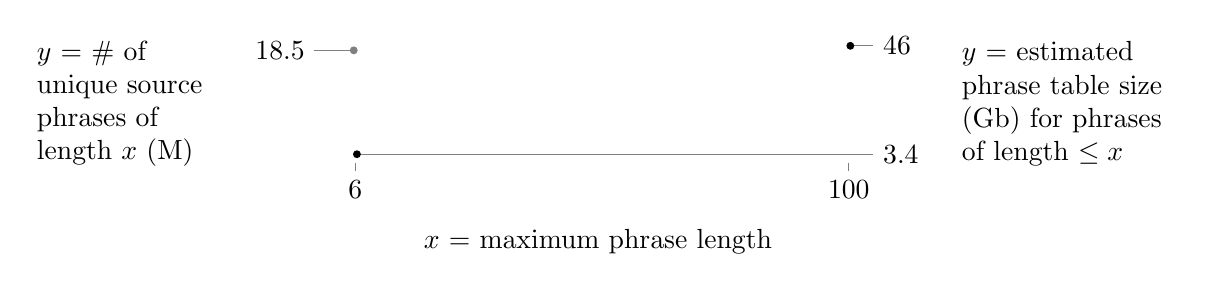
\begin{tikzpicture}[ycomb]
		\node [anchor=east,text width=2.5cm] at (-1,0.75){$y$ = \# of unique source phrases of length $x$ (M)};
		\node [anchor=west,text width=2.7cm]  at (8,0.75) {$y$ = estimated phrase table size (Gb) for phrases of length $\leq x$};

		\draw[gray,thin] (0.42,0.0) -- +(0, -0.1) node [black,anchor=north] {6};
		\draw[gray,thin] (6.68667,0.0) -- +(0, -0.1) node [black,anchor=north] {100};

		\draw[gray,thin] (0.4, 1.42816) -- (-0.1, 1.42816) node [black,anchor=east] {18.5};
		\draw[gray,thin] (0.44, 0.109143) -- (7.0, 0.109143) node [black,anchor=west] {3.4};
		\draw[gray,thin] (6.70667, 1.4858) -- (7.0, 1.4858) node [black,anchor=west] {46};

		\node at (3.5,-1.0) {$x$ = maximum phrase length};
		\draw[gray,thick] plot file {chap-overview/data-ngram-phrases};
		\draw[black,thick] plot file {chap-overview/data-ngram-memory};

		\fill[gray] (0.4, 1.42816) circle (0.05);
		\fill[black] (0.44, 0.109143) circle (0.05);
		\fill[black] (6.70667, 1.4858) circle (0.05);
	\end{tikzpicture}
\end{center}

	\end{center}}
	\figpostamble
	\caption{Number of unique source phrases of different lengths and 
	their cumulative effect on estimated phrase table size.}
	\label{fig:unique_source_phrases}
\end{figure}

If our training data grows large enough, setting a maximum phrase
length might not be enough to prevent our model from outgrowing 
available memory. Phrase table filtering is a popular solution to this.
It is used in batch translation, a common scenario
occurring in optimization or in translation of benchmark
data such as those used in the NIST evaluations.  
After the model is computed, source phrases that
don't appear in the test set are removed along with their
translations and parameters, and only parameters needed to
translate the test data are loaded into memory 
(Figure~\ref{fig:filtering}).  Obviously, this method is limited
to cases where we know the test data in advance, such as 
translation of benchmark data for evaluation purposes.
However, it does allow the system to translate with a somewhat
larger model than can reasonably be stored in main memory.
To alleviate test set dependency, we can also filter on 
other criteria \citep{johnson:2007:emnlp-conll}.

Figure~\ref{fig:filtering} illustrates an inefficiency of filtering.
Although we never require the parameters of the complete model at runtime, 
our parameter estimation step still computes all of them.  
We spend additional time removing many 
of them from the model.  For the large corpora
used in contemporary systems, these steps take many hours.

\citet{Zens:2007:hlt-naacl} relax the
dependence on main memory.  They store their model
in an external prefix tree.  Portions of the tree that are 
needed at runtime are paged in from disk.
This allows the model to scale somewhat beyond the limits of memory.
However, they still must make tradeoffs in order to compute their
model offline.  They impose a strict maximum phrase length.

\figpreamble
\begin{figure}
	\figfontsize{
	\begin{center}
		\begin{tikzpicture}
	\node (mem)[rectangle,rounded corners,fill=lightgray,minimum height=4.0cm,minimum width=2.8cm] at (10,-5.6){};
	\node (corpus)[rectangle,draw,label=90:parallel text,minimum height=2.5cm,minimum width=1.5cm] at (0,0) {};
	\foreach \y in {0.05,0.1,...,2.4}{
		\draw[yshift=-1.2cm] (-0.65,\y) -- (-0.05,\y);
		\draw[yshift=-1.2cm] (0.05,\y) -- (0.65,\y);
	}

	\node (rules)[rectangle,draw,label=90:extracted rules,minimum height=4.0cm,minimum width=0.75cm] at (5,0) {};
	\foreach \y in {0.05,0.1,...,3.9}{
		\draw[xshift=5.0cm,yshift=-1.95cm] (-0.3,\y) -- (-0.05,\y);
		\draw[xshift=5.0cm,yshift=-1.95cm] (0.05,\y) -- (0.3,\y);
	}

	\node (pt)[rectangle,draw,fill=white,label=90:phrase table,minimum height=3.5cm,minimum width=2.20cm] at (10,0) {};
	\foreach \y in {0.05,0.1,...,3.4}{
		\draw[xshift=10.0cm,yshift=-1.7cm] (-1.0,\y) -- (-0.75,\y);
		\draw[xshift=10.0cm,yshift=-1.7cm] (-0.65,\y) -- (-0.4,\y);
		\draw[xshift=10.0cm,yshift=-1.7cm] (-0.3,\y) -- (-0.05,\y);
		\draw[xshift=10.0cm,yshift=-1.7cm] (0.05,\y) -- (0.3,\y);
		\draw[xshift=10.0cm,yshift=-1.7cm] (0.4,\y) -- (0.65,\y);
		\draw[xshift=10.0cm,yshift=-1.7cm] (0.75,\y) -- (1.0,\y);
	}

	\node (filtered pt)[rectangle,draw,fill=white,minimum height=0.75cm,minimum width=2.20cm] at (10,-5.35) {};
	\foreach \y in {0.05,0.1,...,0.7}{
		\draw[xshift=10.0cm,yshift=-5.7cm] (-1.0,\y) -- (-0.75,\y);
		\draw[xshift=10.0cm,yshift=-5.7cm] (-0.65,\y) -- (-0.4,\y);
		\draw[xshift=10.0cm,yshift=-5.7cm] (-0.3,\y) -- (-0.05,\y);
		\draw[xshift=10.0cm,yshift=-5.7cm] (0.05,\y) -- (0.3,\y);
		\draw[xshift=10.0cm,yshift=-5.7cm] (0.4,\y) -- (0.65,\y);
		\draw[xshift=10.0cm,yshift=-5.7cm] (0.75,\y) -- (1.0,\y);
	}

	\draw[->] (corpus.east) -- (rules.west);
	\draw[->] (rules.east) -- (pt.west);

	\node [fill=white,draw,rectangle,rounded corners] at (2.65,0) {\begin{tabular}{c}rule\\extraction\end{tabular}};
	\node [fill=white,draw,rectangle,rounded corners] at (7.0,0) {\begin{tabular}{c}parameter\\estimation\end{tabular}};
	\node (filtering) [fill=white,draw,rectangle,rounded corners] at (10,-2.5) {~~filtering~~};

	\node (input) [rectangle,draw,label=90:input source text] at (2.2,-6.75) {\zh{虽然 北 风 呼啸 , 但 天空 依然 十分 清澈 。}};
	\node (decoder)[rectangle,rounded corners,draw,fill=white] at (10,-6.75) {\begin{tabular}{c}decoding\\algorithm\end{tabular}};

	\draw[->] (pt.south) -- (filtering.north);
	\draw[->] (filtering.south) -- (filtered pt.north);
	\draw[->] (filtered pt.south) -- (decoder.north);
	\draw[->] (input.east) -- (decoder.west);
	\draw[->] (6.0,-6.75) -- (6.0,-2.5) -- (filtering.west);
	\node [fill=white,anchor=south] at (mem.north) {main memory};
	\node [fill=lightgray] at (10.0,-4.2){\begin{tabular}{c}filtered\\phrase table\end{tabular}};
\end{tikzpicture}

	\end{center}}
	\figpostamble
	\caption[Architecture of a table-based decoder with filtering.]{Architecture of a table-based decoder with filtering.  
	Filtering is necessary when the model becomes to big to fit into memory 
	(cf. Figure~\ref{fig:table-based}).}\label{fig:filtering}
\end{figure}


We now describe an architecture that requires neither offline computation
of a full model nor limitation to maximum phrase length.


\section{Translation by Pattern Matching}\label{sec:tbpm}

An alternative to direct representation
comes from work in {\em example-based translation}, sometimes called
{\em memory-based translation} \citep{Nagao:1984:ahi,Sato:1990:coling,Somers:2003:raebmt}.  
Like statistical MT, example-based MT
is a data-driven approach to translation.  However, the two approaches
draw on largely separate research traditions.  As we saw in Chapter~\ref{chap:survey},
a unifying principle in statistical MT is optimization.
It draws largely on methods from machine learning.  In contrast, example-based
translation draws from a number of different disciplines.  These include
statistics, but example-based translation is typically not implemented as 
an exercise in optimization.  \citet{Wu:2005:mtjournal} argues
that its distinguishing characteristic is
treatment of the training data as a runtime library and translation by
analogy, making it similar to case-based reasoning.  In fact,
practitioners of example-based MT are not agreed on a precise characterization 
\citep{Hutchins:2005:mtsummit}, and it is sometimes argued that it subsumes
statistical MT \citep{Somers:2003:raebmt}.

Definitions aside, a clear characteristic of
example-based translation is its view of the training
corpus as a database of examples.  To translate a sentence,
the system searches for matching fragments of text in this database at runtime.  
Subsequent steps are system-specific.  However, we are mainly
interested in the idea of efficient search over a
training corpus.  For this, example-based systems use data structures for
efficient efficient pattern matching \citep{Brown:2004:amta}. 

\citet{Callison-Burch:2005:acl} and \citet{Zhang:2005:eamt} independently
applied pattern matching to phrase-based statistical MT.  
They employ a strategy in which the corpus itself is stored in 
main memory, just as in example-based translation.
To decode a new sentence, the system employs pattern matching to
search for each candidate source phrase
in the source language corpus.  Matching phrases
are extracted along with their aligned target phrases
and scored. The resulting sentence-specific phrase table is 
then used in the decoding algorithm, and subsequently freed from
memory.  In this indirect representation, the
training data itself serves as a proxy for the complete model, and
is queried for model parameters only as needed.
We call this translation by pattern matching.
It is illustrated in Figure~\ref{fig:pattern-matching-architecture}.

\figpreamble
\begin{figure}
	\figfontsize{
	\begin{center}
		\begin{tikzpicture}
	\node (mem)[rectangle,rounded corners,fill=lightgray,minimum height=4.3cm,minimum width=12.6cm] at (5.15,-0.15){};
	\node (corpus)[rectangle,fill=white,draw,label=90:parallel text,minimum height=2.5cm,minimum width=1.5cm] at (0,0) {};
	\foreach \y in {0.05,0.1,...,2.4}{
		\draw[yshift=-1.2cm] (-0.65,\y) -- (-0.05,\y);
		\draw[yshift=-1.2cm] (0.05,\y) -- (0.65,\y);
	}

	\node (rules)[rectangle,fill=white,draw,minimum height=1.5cm,minimum width=0.75cm] at (5,0) {};
	\foreach \y in {0.05,0.1,...,1.45}{
		\draw[xshift=5.0cm,yshift=-0.74cm] (-0.3,\y) -- (-0.05,\y);
		\draw[xshift=5.0cm,yshift=-0.74cm] (0.05,\y) -- (0.3,\y);
	}
	\node [anchor=south] at (rules.north) {\begin{tabular}{c}sentence-specific\\extracted rules\end{tabular}};

	\node (pt)[rectangle,draw,fill=white,minimum height=0.75cm,minimum width=2.20cm] at (10,0) {};
	\foreach \y in {0.05,0.1,...,0.7}{
		\draw[xshift=10.0cm,yshift=-0.36cm] (-1.0,\y) -- (-0.75,\y);
		\draw[xshift=10.0cm,yshift=-0.36cm] (-0.65,\y) -- (-0.4,\y);
		\draw[xshift=10.0cm,yshift=-0.36cm] (-0.3,\y) -- (-0.05,\y);
		\draw[xshift=10.0cm,yshift=-0.36cm] (0.05,\y) -- (0.3,\y);
		\draw[xshift=10.0cm,yshift=-0.36cm] (0.4,\y) -- (0.65,\y);
		\draw[xshift=10.0cm,yshift=-0.36cm] (0.75,\y) -- (1.0,\y);
	}
	\node [anchor=south] at (pt.north) {\begin{tabular}{c}sentence-specific\\phrase table\end{tabular}};

	\draw[->] (corpus.east) -- (rules.west);
	\draw[->] (rules.east) -- (pt.west);

	\node (pm) [fill=white,draw,rectangle,rounded corners] at (2.65,0) {\begin{tabular}{c}pattern matching\\and source-driven\\rule extraction\end{tabular}};
	\node [fill=white,draw,rectangle,rounded corners] at (7.0,0) {\begin{tabular}{c}parameter\\estimation\end{tabular}};

	\node (input) [rectangle,draw] at (2.65,-3.5) {\zh{虽然 北 风 呼啸 , 但 天空 依然 十分 清澈 。}};

	\node (decoder)[rectangle,rounded corners,draw,fill=white] at (10,-1.5) {\begin{tabular}{c}decoding\\algorithm\end{tabular}};

	\draw[->] (pt.south) -- (decoder.north);
	\draw[<-] (decoder.south) -- (10,-3.5) -- (input.east);
	\draw[->] (input.north) -- (pm.south);
	\node [fill=white,anchor=south] at (mem.north) {main memory};

	\node [anchor=south,fill=white] at (input.north) {input source text};

\end{tikzpicture}

	\end{center}}
	\figpostamble
	\caption[Translation by pattern matching.]{Translation by pattern matching.  In this architecture, the complete
	model is no longer bound by what we can fit in main memory, or even what we
	can efficiently compute offline.}\label{fig:pattern-matching-architecture}
\end{figure}

Translation by pattern matching has several potential advantages.

\begin{itemize}
	\item It is possible to scale to large corpora without the tradeoffs 
	required by direct representation.

	\item There is no need to filter the model for a specific test set.  This makes
	translation by pattern matching suitable for online settings where arbitrary
	input is expected.

	\item Where applicable, arbitrarily long phrases can be used, since we generate
	and discard phrase pairs as necessary and do not need to keep them in memory all at once.

	\item Because there is no need to extract, score, and store a complete
	model, it becomes much easier to experiment with grammar parameters
	and features. This is illustrated in Chapter~\ref{chap:scaling}.

\end{itemize}

\noindent These are all potentially valuable benefits.  However, 
while \citet{Callison-Burch:2005:acl} and \citet{Zhang:2005:eamt}
lay the foundation for translation by pattern matching, they leave
some unanswered questions.

\begin{itemize}
	\item It is difficult to include the target-to-source translation
	feature (Equation~\ref{eq:inv-ptp}).  To compute the 
	probability $p(\tilde{f}|\tilde{e})$ we need a count of 
	all source phrases in the corpus that align to the target
	phrase $\tilde{e}$.  This implies that after searching for and
	extracting rules for a source phrase, we must then search for 
	and extract rules for all of its possible target phrases.
	As we will see, the initial search and extraction for the source
	phrase is expensive.  An additional search for target 
	phrases would be onerous, so we sacrifice the feature for efficiency.  
	However, as we saw in Chapter~\ref{chap:survey}, 
	this feature originated in the earliest Bayesian approaches to 
	statistical MT (\textsection\ref{sec:generative-models}), 
	and has since been considered indispensable.  It is not
	clear how a system will fare without it.

	\item The models of \citet{Callison-Burch:2005:acl} and \citet{Zhang:2005:eamt}
	were not optimized for translation accuracy using minimum error rate training
	\citep[see \textsection\ref{sec:minimum-error-rate-training}]{Och:2003:acl}.
	In fact, as we will show, an optimization technique used by their approach
	has an undesirable interaction with the MERT algorithm
	\cite[\textsection\ref{sec:minimum-error-rate-training}]{Och:2003:acl}
	used for optimization.  Therefore, paradoxically, although they can easily exploit 
	very large corpora, neither paper reports state-of-the-art results on 
	benchmark data.\footnote{\citet{Callison-Burch:2005:acl} evaluate on a 
	unique test set, making their results difficult to situate in
	the literature.  \citet{Zhang:2005:eamt} evaluate on the
	NIST 2002 Chinese-English task achieving a BLEU
	score of 17.6.  A comparable phrase-based system achieves a score
	of 34.9 on the same task \citep{DeNeefe:2007:emnlp-conll}.  The latter score is 
	typical of the best models on this data.  Under most circumstances,
	we caution that it is misleading to directly compare self-reported 
	BLEU scores.  Differences in implementation, tokenization, and capitalization 
	can lead to differences of several BLEU points.  However, due to the 
	extreme difference in this case, we can confidently state these are 
	extremely poor results.}  It is therefore unclear whether translation by pattern 
	matching is a viable approach for state-of-the-art 
	results, or merely a clever algorithmic curiosity.

	\item The algorithms could only be applied to phrase-based models based on 
	contiguous phrases.  In Chapter~\ref{chap:survey}, we described an increasingly
	complex progression of models.  Several of these, such as the model of 
	\citet{Chiang:2005:acl,Chiang:2007:cl}, allow translation of discontiguous
	phrases.  The pressures we described above for standard
	phrase-based models are much more acute for these models.  However, the
	method of \citet{Callison-Burch:2005:acl} and \citet{Zhang:2005:eamt}
	does not work for discontiguous phrases.
\end{itemize}

In this chapter and the next, we solve these problems.  In order to 
gain a deeper understanding of them, we first review
the suffix array data structure used to implement
translation by pattern matching (\textsection\ref{sec:suffix_arrays}).  We
also describe source-driven rule extraction
(\textsection\ref{sec:source-driven-rule-extraction}).

\subsection{Pattern Matching and Suffix Arrays}\label{sec:suffix_arrays}

A fundamental task in pattern matching is {\em exact pattern matching} on strings.
We are given a {\em query pattern} $w$ and a {\em text} $T$,
and our goal is to find all occurrences of $w$ in $T$.  Exact
pattern matching has a vast array of applications and many
algorithms have been developed. \citet{Gusfield:1997:book}
gives an excellent introduction, with a focus on algorithms used in 
biological sequence analysis.  

In phrase-based translation, we are given an input sentence of length $J$.
Each of its $J^2$ substrings is a possible source phrase.  We
need to query the source side of the training bitext for each of these
substrings (Figure~\ref{fig:pb-query}).  If we have a fast enough exact
pattern matching algorithm for single query patterns,
we can implement our framework by enumerating all substrings
of the input and searching the training text for each of them.

\figpreamble
\begin{figure}
	\figfontsize{
	\begin{center}
		Input Sentence:
{\em it persuades him and it disheartens him}

~

Query Patterns:
{\em
it, persuades, him, and, disheartens,
it~persuades, persuades~him, him~and, and~it, disheartens~him,
it~persuades~him, persuades~him~and, him~and~it, and~it~disheartens, it~disheartens~him,
it~persuades~him~and, persuades~him~and~it, him~and~it~disheartens, and~it~disheartens~him,
it~persuades~him~and~it, persuades~him~and~it~disheartens, him~and~it~disheartens~him,
it~persuades~him~and~it~disheartens, persuades~him~and~it~disheartens~him,
it~persuades~him~and~it~disheartens~him
}

	\end{center}}
	\figpostamble
	\caption[Example input sentence and resulting query patterns for phrase-based translation.]{Example input sentence and resulting query 
	patterns for phrase-based translation.
	For clarity, all of our pattern matching examples are in
	English, though in practice our source text is Chinese.}
	\label{fig:pb-query}
\end{figure}

To implement fast lookup on the text, we use an indexing data structure
called a {\em suffix array} \citep{Manber:1993:sicomp}.  It 
represents all {\em suffixes} of the text in lexicographical order.
Formally, the $i$th suffix of text $T$ is the substring
beginning at position $i$ and continuing to the end of $T$ (Figure~\ref{fig:text}).
This suffix is uniquely identified by the index $i$ of its first word.
The suffix array $SA_T$ of $T$ is a permutation on the 
set of suffix identifiers $[0,|T|-1]$ 
corresponding to the lexicographical order of the
suffixes (Figure~\ref{fig:suffix-array}).\footnote{Actually,
any total ordering on the tokens can be used.
In our implementation we use the natural order on a
integerized representation of words.}

\figpreamble
\begin{figure}
	\figfontsize{
	\begin{center}
		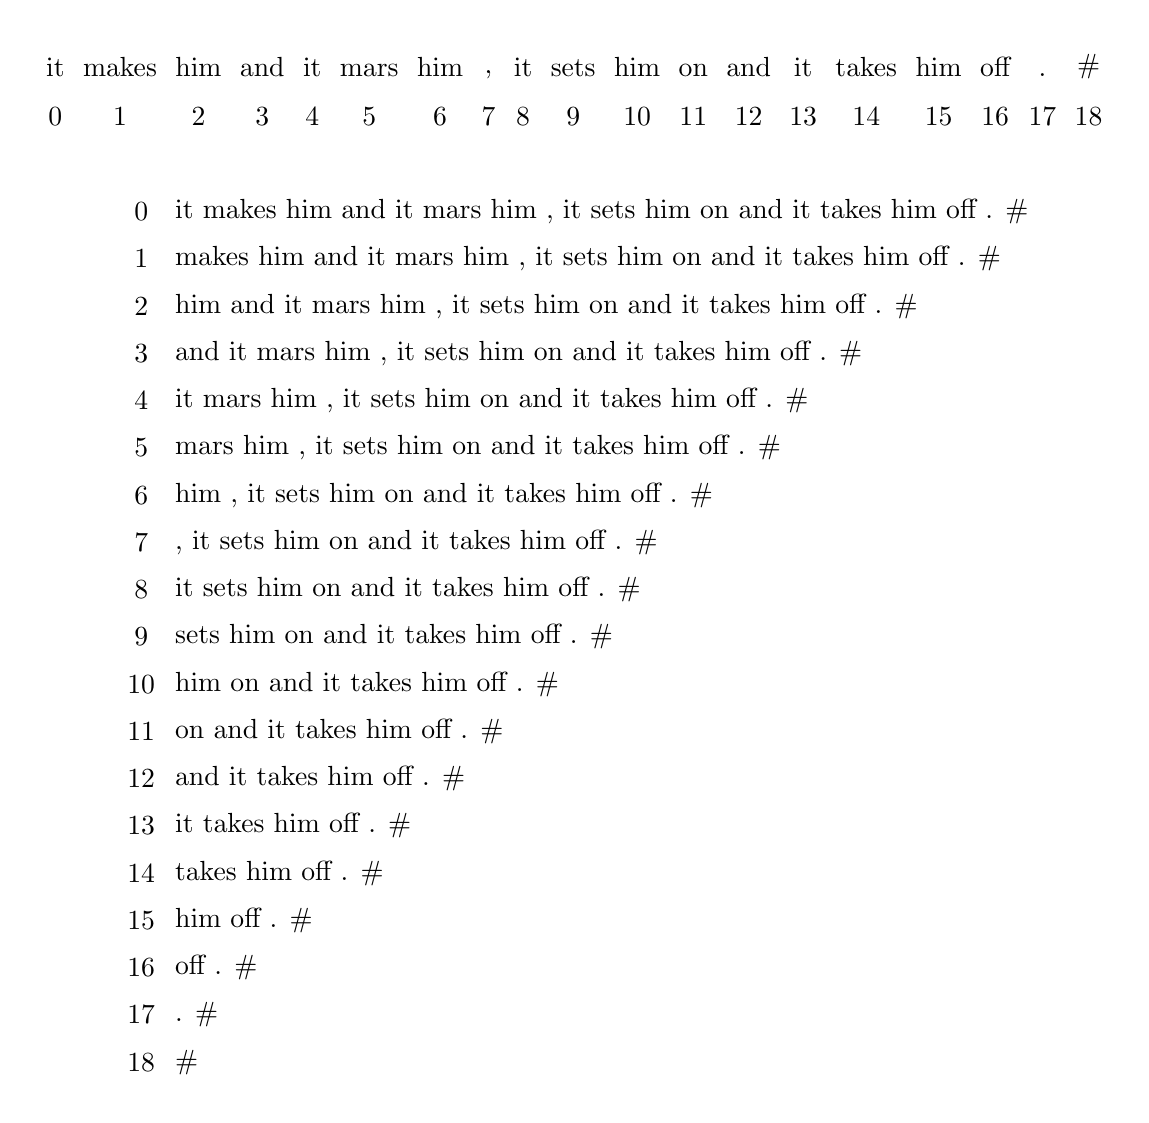
\begin{tikzpicture}
	\matrix (sentence) [nodes={text height=10pt}] at (5.5,7){
	\node {it}; & \node(word){makes}; & \node{him}; & \node{and}; & \node{it}; & \node{mars}; & \node {him}; & \node{,}; & \node{it}; & \node{sets}; & \node{him}; & \node{on}; & \node{and}; & \node{it}; & \node{takes}; & \node{him}; & \node{off}; & \node{.}; & \node{\#};\\
	\node {0}; & \node(num){1}; & \node{2}; & \node{3}; & \node{4}; & \node{5}; & \node {6}; & \node{7}; & \node{8}; & \node{9}; & \node{10}; & \node{11}; & \node{12}; & \node{13}; & \node{14}; & \node{15}; & \node{16}; & \node{17}; & \node{18};\\
	};

	\matrix [nodes={rectangle,minimum size=6mm}] at (0,0){
		\node (suffix 0) {0}; \\
		\node (suffix 1) {1}; \\
		\node (suffix 2) {2}; \\
		\node (suffix 3) {3}; \\
		\node (suffix 4) {4}; \\
		\node (suffix 5) {5}; \\
		\node (suffix 6) {6}; \\
		\node (suffix 7) {7}; \\
		\node (suffix 8) {8}; \\
		\node (suffix 9) {9}; \\
		\node (suffix 10) {10}; \\
		\node (suffix 11) {11}; \\
		\node (suffix 12) {12}; \\
		\node (suffix 13) {13}; \\
		\node (suffix 14) {14}; \\
		\node (suffix 15) {15}; \\
		\node (suffix 16) {16}; \\
		\node (suffix 17) {17}; \\
		\node (suffix 18) {18}; \\
	};
	\node [anchor=west] at (suffix 0.east) {it makes him and it mars him , it sets him on and it takes him off . \#};
	\node [anchor=west] at (suffix 1.east) {makes him and it mars him , it sets him on and it takes him off . \#};
	\node [anchor=west] at (suffix 2.east) {him and it mars him , it sets him on and it takes him off . \#};
	\node [anchor=west] at (suffix 3.east) {and it mars him , it sets him on and it takes him off . \#};
	\node [anchor=west] at (suffix 4.east) {it mars him , it sets him on and it takes him off . \#};
	\node [anchor=west] at (suffix 5.east) {mars him , it sets him on and it takes him off . \#};
	\node [anchor=west] at (suffix 6.east) {him , it sets him on and it takes him off . \#};
	\node [anchor=west] at (suffix 7.east) {, it sets him on and it takes him off . \#};
	\node [anchor=west] at (suffix 8.east) {it sets him on and it takes him off . \#};
	\node [anchor=west] at (suffix 9.east) {sets him on and it takes him off . \#};
	\node [anchor=west] at (suffix 10.east) {him on and it takes him off . \#};
	\node [anchor=west] at (suffix 11.east) {on and it takes him off . \#};
	\node [anchor=west] at (suffix 12.east) {and it takes him off . \#};
	\node [anchor=west] at (suffix 13.east) {it takes him off . \#};
	\node [anchor=west] at (suffix 14.east) {takes him off . \#};
	\node [anchor=west] at (suffix 15.east) {him off . \#};
	\node [anchor=west] at (suffix 16.east) {off . \#};
	\node [anchor=west] at (suffix 17.east) {. \#};
	\node [anchor=west] at (suffix 18.east) {\#};

\end{tikzpicture}

	\end{center}}
	\figpostamble
	\caption[Example of a text and its set of suffixes]{Example of a 
	text and its set of suffixes.  Note that each suffix can be uniquely
	identified by its starting position in the text.
	In keeping with a common convention of the pattern matching literature,
	the text ends with a special
	symbol ({\em \#}) that is distinct from every other symbol in the
	alphabet.}
	\label{fig:text}
\end{figure}

Suffix arrays enable fast exact pattern matching.  Every substring of $T$
is the prefix of a suffix of $T$.  Because $SA_T$ represents
the suffixes in lexicographical order, we can find all occurrences of a 
substring $w$ with binary search.  Every occurrence of $w$ will correspond to exactly one
suffix of $T$, and they will all be found within a contiguous range of $SA_T$.
This range can be identified with a pair of binary searches on the suffix
array.  Specifically, a length-$m$ substring can be found in $O(m + \log |T|)$ time 
\citep{Manber:1993:sicomp}.\footnote{This result requires a bit of algorithmic
subtlety that we ignore here.  In fact, this simple algorithm is not the most
efficient solution.  \citet{Abouelhoda:2004:jda} show that
lookup can be done in optimal $O(m)$ time using some auxiliary data structures.
However, for our purposes $O(m + \log |T|)$ is reasonable.  The latter term, which we
can think of as a corpus-specific constant, is fairly mild.}

\figpreamble
\begin{figure}
	\figfontsize{
	\begin{center}
			\begin{tikzpicture}
		\matrix (sentence) [nodes={text height=10pt}] at (5.5,7){
		\node (word 0) {it}; & 
		\node (word 1) {makes}; & 
		\node (word 2) {him}; & 
		\node (word 3) {and}; & 
		\node (word 4) {it}; & 
		\node (word 5) {mars}; & 
		\node (word 6) {him}; & 
		\node (word 7) {,}; & 
		\node (word 8) {it}; & 
		\node (word 9) {sets}; & 
		\node (word 10) {him}; & 
		\node (word 11) {on}; & 
		\node (word 12) {and}; & 
		\node (word 13) {it}; & 
		\node (word 14) {takes}; & 
		\node (word 15) {him}; & 
		\node (word 16) {off}; & 
		\node (word 17) {.}; & 
		\node (word 18) {\#};\\
		\node (num 0) {0}; & 
		\node (num 1) {1}; & 
		\node (num 2) {2}; & 
		\node (num 3) {3}; & 
		\node (num 4) {4}; & 
		\node (num 5) {5}; & 
		\node (num 6) {6}; & 
		\node (num 7) {7}; & 
		\node (num 8) {8}; & 
		\node (num 9) {9}; & 
		\node (num 10) {10}; & 
		\node (num 11) {11}; & 
		\node (num 12) {12}; & 
		\node (num 13) {13}; & 
		\node (num 14) {14}; & 
		\node (num 15) {15}; & 
		\node (num 16) {16}; & 
		\node (num 17) {17}; & 
		\node (num 18) {18};\\
		};


		\draw[snake=brace,segment amplitude=2mm] (word 2.north west) -- (word 2.north east);
		\draw[snake=brace,segment amplitude=2mm] (word 6.north west) -- (word 6.north east);
		\draw[snake=brace,segment amplitude=2mm] (word 10.north west) -- (word 10.north east);
		\draw[snake=brace,segment amplitude=2mm] (word 15.north west) -- (word 15.north east);

%		\fill[lightgray] (word 2.north west) rectangle (num 2.south east) rectangle (word 2.north east);
%		\fill[lightgray] (word 6.north west) rectangle (num 6.south east) rectangle (word 6.north east);
%		\fill[lightgray] (word 10.north west) rectangle (num 10.south east) rectangle (word 10.north east);
%		\fill[lightgray] (word 15.north west) rectangle (num 15.south east) rectangle (word 15.north east);
%
%		\node [text height=10pt] at (word 2.center) {him};
%		\node [text height=10pt] at (word 6.center) {him};
%		\node [text height=10pt] at (word 10.center) {him};
%		\node [text height=10pt] at (word 15.center) {him};
%		\node [text height=10pt] at (num 2.center) {2};
%		\node [text height=10pt] at (num 6.center) {6};
%		\node [text height=10pt] at (num 10.center) {10};
%		\node [text height=10pt] at (num 15.center) {15};

		\matrix [nodes={rectangle,draw,minimum width=6.5mm,minimum height=6mm}] at (0,0){
			\node (suffix 3) {3}; \\
			\node (suffix 12) {12}; \\
			\node (suffix 2)  [fill=lightgray]{2}; \\
			\node (suffix 15) [fill=lightgray]{15}; \\
			\node (suffix 10) [fill=lightgray]{10}; \\
			\node (suffix 6)  [fill=lightgray]{6}; \\
			\node (suffix 0) {0}; \\
			\node (suffix 4) {4}; \\
			\node (suffix 8) {8}; \\
			\node (suffix 13) {13}; \\
			\node (suffix 1) {1}; \\
			\node (suffix 5) {5}; \\
			\node (suffix 16) {16}; \\
			\node (suffix 11) {11}; \\
			\node (suffix 9) {9}; \\
			\node (suffix 14) {14}; \\
			\node (suffix 7) {7}; \\
			\node (suffix 17) {17}; \\
			\node (suffix 18) {18}; \\
		};

		\node [anchor=west,xshift=6pt] at (suffix 0.east) {it makes him and it mars him , it sets him on and it takes him off . \#};
		\node [anchor=west,xshift=6pt] at (suffix 1.east) {makes him and it mars him , it sets him on and it takes him off . \#};
		\node [anchor=west,xshift=3pt] at (suffix 2.east) {\colorbox{lightgray}{him} and it mars him , it sets him on and it takes him off . \#};
		\node [anchor=west,xshift=6pt] at (suffix 3.east) {and it mars him , it sets him on and it takes him off . \#};
		\node [anchor=west,xshift=6pt] at (suffix 4.east) {it mars him , it sets him on and it takes him off . \#};
		\node [anchor=west,xshift=6pt] at (suffix 5.east) {mars him , it sets him on and it takes him off . \#};
		\node [anchor=west,xshift=3pt] at (suffix 6.east) {\colorbox{lightgray}{him} , it sets him on and it takes him off . \#};
		\node [anchor=west,xshift=6pt] at (suffix 7.east) {, it sets him on and it takes him off . \#};
		\node [anchor=west,xshift=6pt] at (suffix 8.east) {it sets him on and it takes him off . \#};
		\node [anchor=west,xshift=6pt] at (suffix 9.east) {sets him on and it takes him off . \#};
		\node [anchor=west,xshift=3pt] at (suffix 10.east) {\colorbox{lightgray}{him} on and it takes him off . \#};
		\node [anchor=west,xshift=6pt] at (suffix 11.east) {on and it takes him off . \#};
		\node [anchor=west,xshift=6pt] at (suffix 12.east) {and it takes him off . \#};
		\node [anchor=west,xshift=6pt] at (suffix 13.east) {it takes him off . \#};
		\node [anchor=west,xshift=6pt] at (suffix 14.east) {takes him off . \#};
		\node [anchor=west,xshift=3pt] at (suffix 15.east) {\colorbox{lightgray}{him} off . \#};
		\node [anchor=west,xshift=6pt] at (suffix 16.east) {off . \#};
		\node [anchor=west,xshift=6pt] at (suffix 17.east) {. \#};
		\node [anchor=west,xshift=6pt] at (suffix 18.east) {\#};

	\end{tikzpicture}

	\end{center}}
	\figpostamble
	\caption[Suffix array example]{Suffix array for the example text of Figure~\ref{fig:text}.
	We also show the result of a query for the pattern {\em him}.  Note that each occurrence
	is the prefix of a suffix of the corpus, that there is a one-to-one correspondence between
	the occurrences and the suffixes, and that all of the suffixes occur in a contiguous 
	stretch of the array, meaning that we can find them using binary search.}
	 \label{fig:suffix-array}
\end{figure}


\subsection{Source-Driven Phrase Extraction and Scoring}\label{sec:source-driven-rule-extraction}

Once we have found the occurrences of a source phrase, we need to
extract its translations.  If we were computing a direct representation
of the model, we would simply extract all viable phrase pairs from the
sentence in which the source phrase occurs.  However, since we only
need the translation of the source phrase we are interested in,
this is inefficient.  Our goal is to extract only the translation
of the specific source phrase that we have found.  
We call this {\em source-driven phrase extraction}.

Given a source phrase, its target phrase will be the minimal
target span containing all words that are aligned to at least 
one of its words.  To find this span, we simply find the 
minimal and maximal target word indices of all words aligned
to any word in the source phrase.

We are not quite done.  Recall that none of the words in a valid
phrase pair can be aligned to words outside the pair 
(\textsection\ref{sec:supervised-estimation-generative}).
In order to extract the phrase pair,
we must check to see whether this condition is satisfied.
To do this, we invert the previous step and
find the minimal source span that is aligned
to the target span.  If this source span does not match the 
original source phrase, then the target phrase is aligned to
words outside of the source phrase and extraction fails.  Otherwise,
we extract the target phrase.  Under a {\em loose} heuristic \citep{Ayan:2006:acl-coling},
we can also extract target phrases containing any unaligned
target words immediately adjacent to the target span.  Phrase
extraction is illustrated in Figure~\ref{fig:phrase-extraction}.

Once we have collected all of the target phrases that are aligned
to a source phrase, we can compute the source-to-target translation
probabilities and lexical weightings.  For the latter we rely on
a precomputed table of word-to-word translation probabilities computed
from the word-level alignment.

\figpreamble
\begin{figure}
	\figfontsize{
	\begin{center}
		\begin{tikzpicture}
	\renewcommand\currentex[1]{\extractionex{5}{1, 5}{2,...,4}{1/1, 2/2, 3/4, 4/4, 5/5}{#1}}
	\currentex{}
	\node [anchor=south] at (source 3.north) {1. Find source phrase $f_2 f_3 f_4$};
	\path (target 1.south west) -- +(0,-3) coordinate (ex 1 left);
	\begin{scope}[xshift=5cm]
		\currentex{
			\path[style=main phrase] (target 2.north west) rectangle (target 4.south east);
		}
		\node [anchor=south] at (source 3.north) {2. Find target span};
	\end{scope}
	\begin{scope}[xshift=10cm]
		\currentex{
			\fill[main phrase] (source 2.north west) rectangle (target 4.south east);
		}
		\node [anchor=south] at (source 3.north) {3. Find reflected source span};
		\path (target 5.south east) -- +(0,-3) coordinate (ex 1 right);
		\draw[snake=brace,segment amplitude=2mm] (target 4.south east) -- (target 2.south west) 
			node (extract label) [below=2mm,pos=0.5] {4. Extract $f_2 f_3 f_4 / e_2 e_3 e_4$};
	\end{scope}
	\path (extract label.south) -- +(0,-0.15) coordinate (bottom);
	\draw [gray,thin] (bottom) -- (bottom -| ex 1 left) coordinate (label loc);
	\draw [gray,thin] (bottom) -- (bottom -| ex 1 right);
	\node [anchor=south west] at (label loc) {Successful phrase extraction};

	\begin{scope}[yshift=-3.5cm]
		\renewcommand\currentex[1]{\extractionex{5}{1, 5}{2,...,4}{1/3, 2/4, 3/4, 4/2, 5/5}{#1}}
		\currentex{}
		\node [anchor=south] at (source 3.north) {1. Find source phrase $f_2 f_3 f_4$};
		\path (target 1.south west) -- +(0,-3) coordinate (ex 1 left);
		\begin{scope}[xshift=5cm]
			\currentex{
				\path[style=main phrase] (target 2.north west) rectangle (target 4.south east);
			}
			\node [anchor=south] at (source 3.north) {2. Find target span};
		\end{scope}
		\begin{scope}[xshift=10cm]
			\currentex{
				\fill[main phrase] (source 1.north west) 
					-- (source 4.north east) 
					-- (target 4.south east) 
					-- (target 2.south west)
					-- (target 2.north west)
					-- (source 1.south west)
					--cycle;
			}
			\node [anchor=south] at (source 3.north) {3. Find reflected source span};
			\node (extract label) [anchor=north,text width=5cm] at (target 3.south) {\begin{center}4. Extraction fails because reflected source span exceeds original source phrase\end{center}};
			\path (target 5.south east) -- +(0,-3) coordinate (ex 1 right);
		\end{scope}
		\path (extract label.south) -- +(0,-0.15) coordinate (bottom);
		\draw [gray,thin] (bottom) -- (bottom -| ex 1 left) coordinate (label loc);
		\draw [gray,thin] (bottom) -- (bottom -| ex 1 right);
		\node [anchor=south west] at (label loc) {Unsuccessful phrase extraction};
	\end{scope}

	\begin{scope}[yshift=-7.6cm]
		\renewcommand\currentex[1]{\extractionex{5}{1, 5}{2,...,4}{2/2, 3/4, 4/4}{#1}}
		\currentex{}
		\node [anchor=south] at (source 3.north) {1. Find source phrase $f_2 f_3 f_4$};
		\node (explanation) [anchor=north,below=4mm,text width=4.5cm] at (target 4.south) {\begin{center}Under the loose heuristic, unaligned words to the left and right of the target span may be part of a phrase.\end{center}};
		\path (target 1.south west) -- +(0,-3) coordinate (ex 1 left);
		\begin{scope}[xshift=5cm]
			\currentex{
				\path[style=main phrase] (target 2.north west) rectangle (target 4.south east);
			}
			\node [anchor=south] at (source 3.north) {2. Find target span};
			\draw[->,gray,thin] (explanation.east) ..controls +(0.4,0) .. (target 1.south);
			\draw[->,gray,thin] (explanation.east) ..controls +(3.2,0) .. (target 5.south);
		\end{scope}
		\begin{scope}[xshift=10cm]
			\currentex{
				\fill[main phrase] (source 2.north west) rectangle (target 4.south east);
			}
			\node [anchor=south] at (source 3.north) {3. Find reflected source span};
			\draw[snake=brace,segment amplitude=2mm] (target 4.south east) -- (target 2.south west) 
				node[below=2mm,pos=0.5] {4. Extract $f_2 f_3 f_4 / e_2 e_3 e_4$};
			\draw[snake=brace,raise snake=8mm,segment amplitude=2mm] (target 4.south east) -- (target 1.south west) 
				node[below=10mm,pos=0.5] {5. Extract $f_2 f_3 f_4 / e_1 e_2 e_3 e_4$};
			\draw[snake=brace,raise snake=16mm,segment amplitude=2mm] (target 5.south east) -- (target 2.south west) 
				node[below=18mm,pos=0.5] {6. Extract $f_2 f_3 f_4 / e_2 e_3 e_4 e_5$};
			\draw[snake=brace,raise snake=24mm,segment amplitude=2mm] (target 5.south east) -- (target 1.south west) 
				node(extract label) [below=26mm,pos=0.5] {7. Extract $f_2 f_3 f_4 / e_1 e_2 e_3 e_4 e_5$};
			\path (target 5.south east) -- +(0,-3) coordinate (ex 1 right);
		\end{scope}
		\path (extract label.south) -- +(0,-0.15) coordinate (bottom);
		\path (bottom) -- (bottom -| ex 1 left) coordinate (label loc);
		\path (bottom) -- (bottom -| ex 1 right);
		\node [anchor=south west] at (label loc) {Phrase extraction using the {\em loose} heuristic};
	\end{scope}
\end{tikzpicture}

	\end{center}}
	\figpostamble
	\caption{Examples of source-driven phrase extraction.}
	\label{fig:phrase-extraction}
\end{figure}

The complexity of extraction and scoring is linear in the number
of occurrences of a source phrase.  In Figure~\ref{fig:ngram-histogram},
we see that the vast majority of source phrases occur only a handful
of times in our corpus.  However, a small handful of source phrases occur
hundreds of thousands of times in our corpus.  Extracting all of these
examples would be extremely expensive.  \citet{Callison-Burch:2005:acl} and 
\citet{Zhang:2005:eamt} counteract this problem with sampling.
Rather than extracting a translation for every occurrence of a source phrase, they 
place a cap on the number of of examples.  Both groups
arrived at a sample size of 100 via experimentation.\footnote{This sample
is obviously small for the handful of phrases occurring
tens or hundreds of thousands of times.  It is perhaps surprising
that this should work as well as the full data.
However, \citet{Och:2005:wpt} and \citet{Federico:2006:smt} show that 
phrase translation probabilities can be stored in four bits
without loss of precision, meaning that they are in fact very crude
even when computed from complete data.}
It is unclear how sampling interacts with the minimum error 
rate training algorithm.  We discuss this in more detail below.

\figpreamble
\begin{figure}
	\figfontsize{
	\begin{center}
		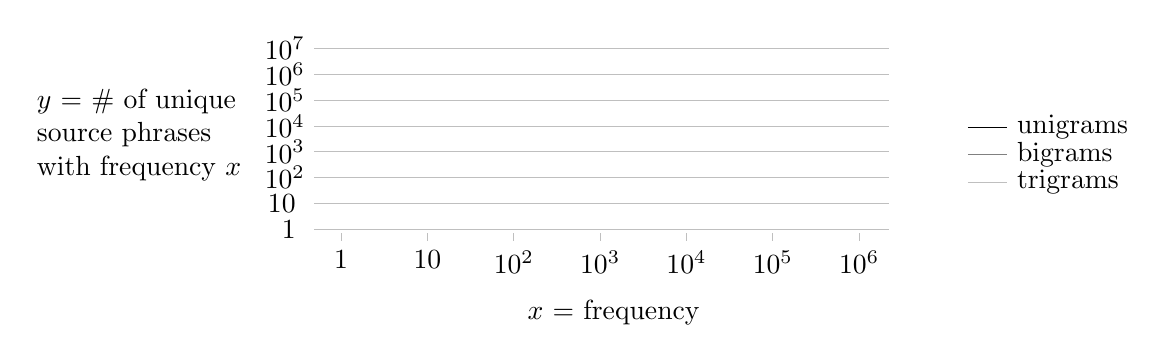
\begin{tikzpicture}
	\node [anchor=east,text width=2.7cm] at (-1,1.25){$y$ = \# of unique source phrases with frequency $x$};

	\draw[lightgray,very thin] (-0.3, 0.05    ) node[anchor=east,black] {$1~   $}-- +(7.3,0);
	\draw[lightgray,very thin] (-0.3, 0.378941) node[anchor=east,black] {$10~  $}-- +(7.3,0);
	\draw[lightgray,very thin] (-0.3, 0.707881) node[anchor=east,black] {$10^2$}-- +(7.3,0);
	\draw[lightgray,very thin] (-0.3, 1.03682 ) node[anchor=east,black] {$10^3$}-- +(7.3,0);
	\draw[lightgray,very thin] (-0.3, 1.36576 ) node[anchor=east,black] {$10^4$}-- +(7.3,0);
	\draw[lightgray,very thin] (-0.3, 1.6947  ) node[anchor=east,black] {$10^5$}-- +(7.3,0);
	\draw[lightgray,very thin] (-0.3, 2.02364 ) node[anchor=east,black] {$10^6$}-- +(7.3,0);
	\draw[lightgray,very thin] (-0.3, 2.35259 ) node[anchor=east,black] {$10^7$}-- +(7.3,0);
	
	\node at (3.5,-1.0) {$x$ = frequency};
	\draw[black,thick,ycomb] plot file {chap-overview/data-unigram-histogram};
	\draw[gray,thick,ycomb] plot file {chap-overview/data-bigram-histogram};
	\draw[lightgray,thick,ycomb] plot file {chap-overview/data-trigram-histogram};
	\draw[lightgray, thin] (0.04000, 0.0) -- +(0,-0.1) node [anchor=north,black] {$1  $};
	\draw[lightgray, thin] (1.13647, 0.0) -- +(0,-0.1) node [anchor=north,black] {$10$};
	\draw[lightgray, thin] (2.23294, 0.0) -- +(0,-0.1) node [anchor=north,black] {$10^2$};
	\draw[lightgray, thin] (3.32941, 0.0) -- +(0,-0.1) node [anchor=north,black] {$10^3$};
	\draw[lightgray, thin] (4.42588, 0.0) -- +(0,-0.1) node [anchor=north,black] {$10^4$};
	\draw[lightgray, thin] (5.52235, 0.0) -- +(0,-0.1) node [anchor=north,black] {$10^5$};
	\draw[lightgray, thin] (6.61881, 0.0) -- +(0,-0.1) node [anchor=north,black] {$10^6$};
	
	\draw (8,1.35) -- +(0.5,0) node [black,anchor=west] {unigrams};
	\draw[gray] (8,1.0) -- +(0.5,0) node [black,anchor=west] {bigrams};
	\draw[lightgray] (8,0.65) -- +(0.5,0) node [black,anchor=west] {trigrams};
\end{tikzpicture}

	\end{center}}
	\figpostamble
	\caption[Histogram of source phrase frequencies.]{Histogram of source phrase frequencies, up to length three (double logscale).}
	\label{fig:ngram-histogram}
\end{figure}

\section{Bringing Performance up to the State of the Art}\label{sec:getting-to-state-of-the-art}

We need to address two questions.  The first is the importance
of the target-to-source phrase translation feature.  This feature
is often assumed to be important to the success of phrase-based-systems.
However, a feature selection experiment by 
\citet{Lopez:2006:amta} suggests that several of the 
standard features were less important than previously thought.  In 
particular, source-to-target feature and target-to-source features 
appeared to be redundant.  Since our system can compute the former
feature, we hope that it will not need the latter.  This question is
answered empirically in \textsection\ref{sec:overview-results}.

A second concern is the application of minimum error rate training
\cite[MERT,][\textsection\ref{sec:minimum-error-rate-training}]{Och:2003:acl}.
Neither \citet{Callison-Burch:2005:acl} nor \citet{Zhang:2005:eamt}
applied it to their models.

A standard approach to sampling in statistical models, 
{\em random sampling}, interacts with the MERT algorithm.  Recall
that the MERT algorithm works by iteratively collecting $n$-best
hypotheses and their feature values.  These are used to compute 
an approximation to the error surface.  A problem with random
sampling is that it causes the feature values for a hypothesis 
to vary between different runs of the system.  This is especially
problematic if the system produces the same hypothesis with different
features during different iterations of the algorithm.  In this
case, the algorithm views these as separate hypotheses.  We found
that, under this strict interpretation, the algorithm would never
converge, because it would never meet the convergence criterion
that no new hypotheses be added in an iteration.  To solve this
problem, we modified the algorithm so that a hypothesis was
not considered new if it had been seen before with different weights.
However, this leads to a new problem: which set of weights should
we choose for the hypothesis?  We decided to take the first set
of weights that had been seen with the hypothesis.  Using this
definition, the algorithm eventually terminates. However, on average
it took twice as many iterations as it did for a standard decoder.

To resolve this issue, we used deterministic sampling.
Whenever a source phrase occurs more frequently than the maximum sample
size, we take our samples at uniform intervals over the set
of locations returned by the suffix array.  With this strategy
in place, hypotheses receive the same feature weights between different
runs of the decoder, the results are deterministic, and the MERT
algorithm converges at the same rate as it does without sampling.

\section{Results}\label{sec:overview-results}

We experimented on Chinese to English translation
in the newswire domain.  Our training data consisted 
of over 1 million sentences compiled from various corpora
provided by the Linguistic Data Consortium.  The corpus is roughly the same as the
one used for large-scale experiments by \citet{Chiang:2005:hlt}.
To generate alignments, we used GIZA++ \citep{Och:2003:cl}.
We symmetrized bidirectional alignments using the grow-diag-final-and
heuristic \citep{Koehn:2003:naacl}.  Each configuration of the system was
separately optimized on the NIST 2003 
Chinese-English test set (919 sentences) using
minimum error rate training 
\citep[\textsection\ref{sec:minimum-error-rate-training}]{Och:2003:acl}. 
We measure translation accuracy using the NIST implementation
of case-insensitive BLEU.\footnote{ftp://jaguar.ncsl.nist.gov/mt/resources/mteval-v11b.pl}
We test on the NIST 2005 Chinese-English test set (1082 sentences).

For our algorithms, we also measure the computational
overhead required to search for, extract, and score rules.
We report the average time required
per sentence on the NIST 2003 data.  All experiments were
performed on identical time-shared cluster machines 
with 8 gigabytes of memory and two dual-core 3GHz Xeon 
processors running Red Hat linux 2.6.9.  
To minimize discrepancies caused by CPU
load, we obtained exclusive use of the machines during 
timing runs.

Our decoder is Pyro, a clone of the Pharaoh decoder
written by David Chiang in the interpreted language 
Python.  We implemented the suffix array extensions in 
Pyrex, a language for writing 
compiled C extensions to Python.  For speed, we compile
our suffix array and other data structures offline 
into memory-mapped files, which are then read at decoder
initialization.
This takes only a few seconds, so the
amortized cost over our data is negligible.\footnote{
In fact, this is the same approach taken by \citet{Zens:2007:hlt-naacl}
for their direct representation.}

\subsection{Baseline System Results}

Our first experiment measures the impact of losing
the target-to-source translation feature (Equation~\ref{eq:inv-ptp}).
We did this using a standard direct representation of the phrase
table using prefix trees, with a phrase length limit of four.

We noticed during development that the phrase count
feature seemed to be minimally important.  Therefore, we
ran the experiments without this feature as well.  This
can be thought of as a kind of manual model selection.
The results are shown in Table~\ref{table:model-selection}.
We see a slight drop in accuracy when we lose the target-to-source
translation feature, but it is not statistically significant.
This indicates that removing the feature is not harmful to
translation accuracy.

\figpreamble
\begin{table}
	\begin{center}
	\begin{tabular}{lc}
		Configuration & BLEU \\ \hline
		baseline with standard eight features & 28.6 \\
		baseline without target-to-source translation feature & 28.3 \\
		baseline without target-to-source translation or phrase count features & 28.2 \\
		baseline without phrase count feature & 28.1 \\
	\end{tabular}
	\end{center}
	\figpostamble
	\caption{Baseline system results compared with systems missing one or more features.}
	\label{table:model-selection}
\end{table}

\subsection{Translation by Pattern Matching Results}

Our next experiment was designed to see if translation by 
pattern matching was a viable replacement for
phrase tables.  In order to make the comparison as fair as
possible, we enforced the same length restriction on phrases
as in the baseline model (Experiments with longer phrases
are in Chapter~\ref{chap:scaling}).  Therefore, the translation
model is nearly the same as in the baseline system.  The only
differences are in the missing target-to-source feature and
the fact that the source-to-target feature is computed by
sampling.

To measure the speed/accuracy tradeoff, we ran the system using
several different sample sizes.  We limited the maximum sample 
size to 800, because larger sizes would have been prohibitively
slow.  For each sample size we were curious
about what fraction of the phrase table was computed
via sampling.  We include the percentage of rules computed by
sampling out of the total number of rules computed.  
These statistics were measured on the development set.

Results are given in Table~\ref{table:overview-results}.  Several 
conclusions are evident.  The first is that translation by pattern 
matching is viable as a replacement for phrase tables. 
Neither \citet{Callison-Burch:2005:acl} and \citet{Zhang:2005:eamt}
matched state-of-the-art performance on a standard benchmark, but our
careful consideration of sampling and minimum error rate training make this possible.
Although the results for the table-based system are slightly higher,
the difference is not statistically significant.  A second result
is that a surprisingly large fraction of the model is computed
by sampling, well over half even for sample sizes giving the best
performance.  Finally, we see that accuracy plateaus once
the sample size reaches about 300.  This essentially confirms the
results of \citet{Callison-Burch:2005:acl} and \citet{Zhang:2005:eamt},
although our best sample size is slightly larger than their
suggested value of 100, which did not fare quite as well.

\figpreamble
\begin{table}
	\begin{center}
		\begin{tabular}{rccc}
			Sample size & \% sampled & time (s)  & BLEU \\ \hline
			{\bf Baseline} & -- & -- & {\bf 28.6} \\
			0  & -- & 0.0094 & -- \\
			10 & 75 & 0.0543 & 25.0 \\
			25 & 67 & 0.0910 & 26.4 \\
			50 & 62 & 0.1447 & 27.6 \\
			100 & 56 & 0.2198 & 27.7 \\
			200 & 51 & 0.3476 & 28.0 \\
			300 & 48 & 0.5216 & 28.4 \\
			{\bf 400} & {\bf 45} & {\bf 0.5557} & {\bf 28.6} \\
			500 & 44 & 0.6492 & 28.5 \\
			800 & 40 & 0.9139 & 28.4 \\
		\end{tabular}
	\end{center}
	\figpostamble
	\caption[Effect of different sample sizes on translation speed and translation accuracy.]{Effect of different sample sizes on translation speed and translation accuracy. We show in column two the percentage of the ruleset that was computed by sampling.  We include a sample size of zero to show the time required for lookup without phrase extraction or scoring.  For comparison, we also show the baseline system using prefix trees and the full feature set from Table~\ref{table:model-selection}.}
	\label{table:overview-results}
\end{table}

\subsection{Analysis of Memory Use}

Our implementation maps each source and target word to a unique 32-bit
integer.  To implement the algorithms, we require several memory-resident
data structures.

\begin{itemize}
	\item The source text $F$ is an array of integers.  Its length is
	dependent on the number of tokens in the source text.  We also
	include special tokens representing both the end of sentence and
	the end of the text.
	\item The target text $E$ is represented in the same way as the source
	text.
	\item The suffix array $SA_F$ is an array of integers.  Its length
	is identical to the length of the target text.
	\item The alignment is an array of integers.  Its length is identical
	to the number of alignment links.
	\item We keep an array of target sentence numbers, allowing us to 
	map from tokens to sentence number in constant time.
	\item We keep a compact array of word-to-word translation probabilities
	in order to compute lexical weighting scores.
\end{itemize}

These data structures are quite compact.  On our data, they require
a little less than 650 megabytes.  In contrast a phrase table may require 
several gigabytes.  We illustrated this using estimates in 
\textsection\ref{sec:phrase-tables}, and we will describe a real
example of a very large phrase table in \textsection\ref{sec:tera-scale-model}.

\section{Conclusions}\label{sec:overview-conclusions}

We have introduced translation by pattern matching, an algorithmic
solution to the problem of translation model scaling.  We have surveyed
past work, identified shortcomings, and overcome them to produce a system
that reproduces state-of-the-art performance in phrase-based translation.
This exercise is a warm-up for more complex models that improve on the standard
phrase-based model.  In the next chapter, we will show how translation
by pattern matching can be applied to these models.





